\documentclass[letterpaper,12pt]{article}
\usepackage[utf8]{inputenc}
\usepackage{fullpage}
\usepackage{courier}
\usepackage[margin=0.75in]{geometry}
\usepackage{listings}
\usepackage{color}
\usepackage{graphicx}
\usepackage[width=4in]{caption}
\usepackage{hyphenat}

% Format a sectionless paragraph
\newcommand*\unparagraph{
	\par
	\nopagebreak
	\vskip3.25ex plus1ex minus.2ex
	\noindent
}

% define extra colors
\definecolor{dkgreen}{rgb}{0,0.6,0}
\definecolor{purple}{RGB}{159,0,197}

% define the code listing format
\lstset{
	language=C++,
	basicstyle=\ttfamily,
	backgroundcolor=\color{white},
	showspaces=false,
	showstringspaces=false,
	frame=none,
	tabsize=3,
	keywordstyle=\color{purple},
	commentstyle=\color{dkgreen},
	stringstyle=\color{blue},
	escapeinside={\%*}{*)}
}

% Define the title/header
\title{\Large CS 1428\\Final} 
\author{Jared Wallace}
\date{}

\begin{document}

\maketitle

\section*{Multiple Choice (2 points each)}

\begin{enumerate}
   \item Which of the following is a valid variable name?
      \begin{enumerate}
         \item \#myFlyVar
         \item amount\_ordered
         \item 25lighters
         \item !0nMyDr3ss3r
      \end{enumerate}
   \item If I want to use input and output to the screen (console) what library do I need?
      \begin{enumerate}
         \item \#include $<$cmath$>$
         \item \#include $<$fstream$>$
         \item \#include $<$cstdlib$>$
         \item \#include $<$iostream$>$
      \end{enumerate}
   \item If I want to read in input from a file of indeterminate size, which loop should I use?
      \begin{enumerate}
         \item for loop
         \item while loop
         \item do while loop
      \end{enumerate}
   \item What's so special about c-strings?
      \begin{enumerate}
         \item They use less memory than regular strings
         \item They are easier to use than regular strings
         \item C is for cookie, and that's good enough for me
         \item They must have a null terminator
      \end{enumerate}

\begin{figure}[ht!]
	\centering
	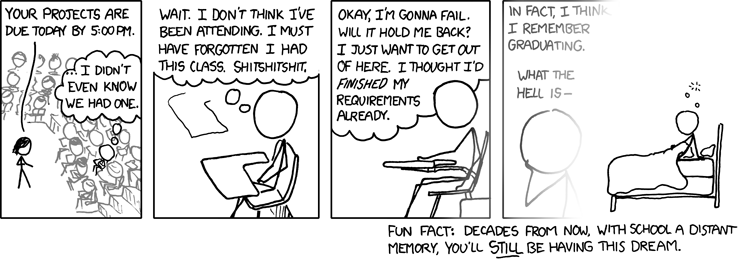
\includegraphics[width=5in]{students.png}
\end{figure}
\newpage
\section*{Harder Multiple Choice (4 points each)}

   \item What is the value of \textbf{problems} after the following snippet?
      \begin{lstlisting}[basicstyle=\footnotesize\ttfamily]
      int problems = 99;
      int money = 500;
      for (int i = 0; i < 3; i++)
      {
         temp = problems;
         problems += money;
         money = temp;
      }
      \end{lstlisting}
      \begin{enumerate}
         \item Problems = 1297
         \item Problems = 999
         \item Problems = 1995
         \item Screw this crap, this ain't math class
      \end{enumerate}
   \item What result is returned from this function if random\_number = 15?
      \begin{lstlisting}[basicstyle=\footnotesize\ttfamily]
      float divide_and_conquer(int random_number)
      {
         return random_number / 6;
      }
      \end{lstlisting}
      \begin{enumerate}
         \item I'd like to use a lifeline
         \item 2.5
         \item Purple
         \item 2
      \end{enumerate}
\section*{True/False (2 points each)}
   \item Arrays always pass by default for all intents and purposes
      \begin{enumerate}
         \item True
         \item False
      \end{enumerate}
   \item When we call a function, we need to provide [] after the variable if it's an array
      \begin{enumerate}
         \item True
         \item False
      \end{enumerate}
   \item Functions must ALWAYS return a value
      \begin{enumerate}
         \item True
         \item False
      \end{enumerate}
   \item Code should never be documented; if it's hard to write, it should be hard to read
      \begin{enumerate}
         \item True
         \item False
      \end{enumerate}

\begin{figure}[ht!]
	\centering
	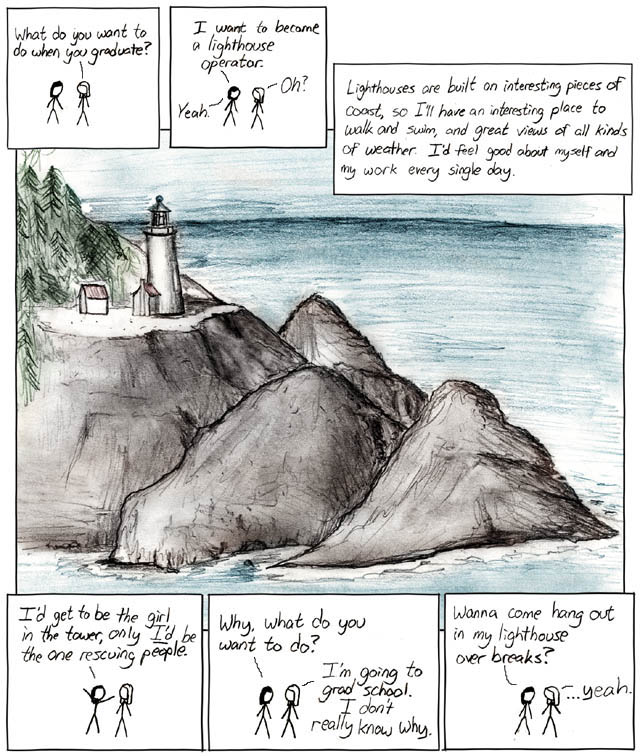
\includegraphics[width=5in]{graduation.jpg}
\end{figure}
\newpage

\section*{Debugging (points vary)}
   \item 5 errors, 2 points apiece. Circle and explain all errors. Ignore style issues.
      \begin{lstlisting}[basicstyle=\footnotesize\ttfamily]
      void main()
      {
         int average,
             sum;
         for (i = 0; i < 10; i++)
            sum += i;
         average = sum/i;
         cout >> "Average is: " >> average;
         return;
      }
      \end{lstlisting}
   \item 3 errors, 2 points apiece.
      \begin{lstlisting}[basicstyle=\footnotesize\ttfamily]
      void populate_array(int [])
      int main()
      {
         int myArray[20];
         populate_array(myarray[]);
         for (int i = 0; i < 20; i++)
            cout << myArray;
         return 0;
      }
      \end{lstlisting}

\begin{figure}[ht!]
	\centering
	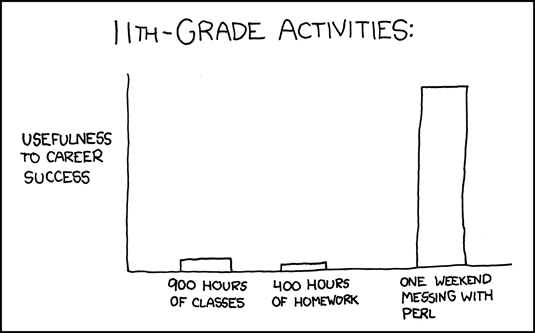
\includegraphics[width=5in]{11th_grade.png}
\end{figure}
\newpage

\section*{Code tracing (20 points)}
   \item What is the exact output of the following C++ code snippet?
      (You may show your work for partial credit, pay attention to how a variable is passed—its position and whether or not it’s pass by reference.)
   \begin{lstlisting}[basicstyle=\footnotesize\ttfamily]
      #include<iostream>

      using namespace std;

      void function1 (int , double);
      void function2 (double &a, int &b);

      int main()
      {
         int x = 7;
         double y = 8.6;

         cout << x << " " << y << endl;
         function1(x, y);
         cout << x << " " << y << endl;
         function2(y, x);
         cout << x << " " << y << endl;

         return 0;
      }

      void function1 (int x, double y)
      {
         cout << x << " " << y << endl;
         x = 0;
         y = 10;
         cout << x << " " << y << endl;
      }

      void function2 (double &a, int &b)
      {
         cout << a << " " << b << endl;
         a = 115.2;
         b = 4;
         cout << a << " " << b << endl;
      }
   \end{lstlisting}
\newpage

\section*{Coding (points as marked)}

   \item Write the C++ code for a void function to print the values in an array to the screen.
      The array is called MaxValues, it contains 393 doubles, and you may assume it has been properly declared.
      DO NOT write the entire program, just this function. (10 points)
\vspace{55mm}
   \item Write a structure called EmployeeRecord with the following fields: (10 points)
      \begin{description}
         \item ID (array of 5 chars)
         \item First (array of 10 chars)
         \item Last (array of 20 chars)
         \item PayRate (float)
      \end{description}
\vspace{55mm}

\begin{figure}[ht!]
	\centering
	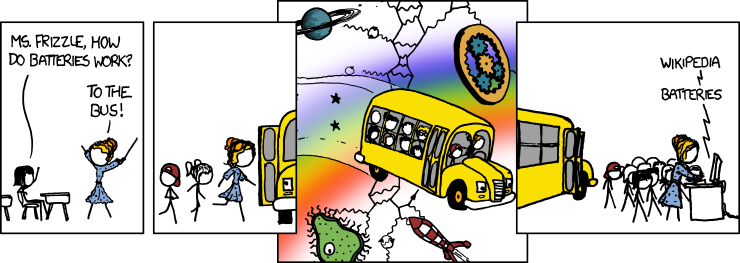
\includegraphics[width=5in]{magic_school_bus.png}
\end{figure}
\newpage
   \item Write a short C++ program that conforms to the following specifications: (15 points)
      \begin{description}
         \item Read a series of numbers in from a file called "input.txt". These represent final grades for a CS 1428 class.
         \item Find the lowest and the highest grades and display them to the screen, along with the average grade.
         \item Hints: This is quite similar to one of your lab assignments. Be sure to use a counter variable to keep
            track of the quantity of grades. You may choose to use functions if you wish.
      \end{description}
\end{enumerate}

\end{document}
